% [Overleaf] https://www.overleaf.com/read/jpkrbtdmyyjc
% [YouTube] https://youtu.be/6ytqbMbTcuQ
% [GitHub] https://github.com/nobucshirai/infona2020_slide_11
\documentclass[dvipdfmx,aspectratio=169,20pt]{beamer}
\usepackage{bxdpx-beamer}

% Beamer theme
\usetheme{Boadilla}

%%%%% JAPANESE FONT SETTINGS %%%%%
\usepackage[utf8]{inputenc}
\usepackage{pxjahyper}
\renewcommand{\kanjifamilydefault}{\gtdefault} % for Gothic Japanese fonts
\newcommand{\myfontsetting}[3]{{\fontsize{#1}{#2}\selectfont #3}}
\usepackage[deluxe,uplatex]{otf} % needed to use super bold Japanese fonts
\usepackage[unicode,noto-otc]{pxchfon} % needed to use super bold Japanese fonts
%%%%%%%%%%%%%%%%%%%%%%%%%%%%%%%%%%

%%%%% SETTINGS FOR MATH SYMBOLS %%%%%
\usepackage{amsmath,amssymb}
\usepackage{bm}
%\usepackage{graphicx}
\usepackage{latexsym}
\usefonttheme{professionalfonts} % use Serif fonts for equations
%%%%%%%%%%%%%%%%%%%%%%%%%%%%%%%%%%%%%

\usepackage{fancybox,ascmac}
\usepackage{url}
\usepackage[many]{tcolorbox}

%%%%% ALGORITHM SETTING %%%%%
\usepackage{algorithm}
\usepackage[noend]{algorithmic}
\algsetup{linenosize=\color{fg!50}\fontsize{8pt}{8pt}\selectfont}
\renewcommand\algorithmicdo{\bfseries :}
\renewcommand\algorithmicthen{\bfseries :}
\renewcommand\algorithmicrequire{\textbf{Input:}}
\renewcommand\algorithmicensure{\textbf{Output:}}
\renewcommand{\algorithmicprint}{\textbf{break}}
%%%%%%%%%%%%%%%%%%%%%%%%%%%%%
\definecolor{myblue1}{RGB}{45,130,200}
\definecolor{my}{RGB}{26,89,142}
\setbeamertemplate{navigation symbols}{}
\setbeamercolor*{structure}{fg=myblue1,bg=blue}
\setbeamercolor{block title}{fg=myblue1!50!black}
\setbeamercolor*{block title example}{fg=white,bg=myblue2}
\setbeamercolor*{palette primary}{use=structure,fg=white,bg=structure.fg}
\setbeamercolor*{palette secondary}{use=structure,fg=white,bg=structure.fg!75!black}
\setbeamercolor*{palette tertiary}{use=structure,fg=white,bg=structure.fg!50!black}
\setbeamercolor*{palette quaternary}{fg=black,bg=myblue1}

\setbeamerfont{alerted text}{series=\bfseries}
\setbeamerfont{section in toc}{series=\mdseries}
\setbeamerfont{frametitle}{size=\Large,series=\bfseries}
\setbeamerfont{title}{size=\LARGE,series=\bfseries}
\setbeamerfont{date}{size=\small}

\setbeamertemplate{block title}[shadow=false]
\setbeamertemplate{blocks}[rounded][shadow=false]

%%%%% BEAMER FOOTLINE SETTINGS %%%%%%
\setbeamertemplate{footline}[frame number]{}
\setbeamerfont{footline}{size=\bf\footnotesize\small}
%%%%%%%%%%%%%%%%%%%%%%%%%%%%%%%%%%%%%

%%%%% BEAMER ITEM SETTINGS %%%%%
\setbeamertemplate{itemize item}[circle]
\setbeamertemplate{itemize subitem}[triangle]
\setbeamertemplate{enumerate item}[circle]
%%%%%%%%%%%%%%%%%%%%%%%%%%%%%%%%

\begin{document}

%%%%%%%%%%%%%%%%%%%%%%%%%%%%%%%%
\begin{frame}
%%%%% START_TAG B %%%%%
%\noindent{\bf X-B.}
\frametitle{[問題] X-B (1)}

\myfontsetting{18pt}{20pt}{
I\hspace{-.1em}X-Bの表1にあるデータをそれぞれのステータスが平均が0、分散が1となるように正規化するプログラムを作成し、正規化されたデータを元にI\hspace{-.1em}X-B表1に相当する表を作成せよ。値は有効数字4桁で5桁目を四捨五入して求めよ。%\\
}
\end{frame}
%%%%%%%%%%%%%%%%%%%%%%%%%%%%%%%%
\begin{frame}
\frametitle{[問題] X-B (2)}

\myfontsetting{18pt}{20pt}{
問1で正規化したデータの3次元ベクトル空間の基底を I\hspace{-.1em}X-B および X-A で求めた3つの固有ベクトルに置き換え、新しい基底での座標を求めてI\hspace{-.1em}X-B表1に相当する表を作成せよ。値は有効数字4桁で5桁目を四捨五入して求めよ。%\\
}\\
\myfontsetting{12pt}{12pt}{
※ 問1, 2において表は手書き作っても良いし、プログラムの出力をコピー\&ペーストしたものでも良い。
}
%%%%% END_TAG B %%%%%
\end{frame}
%%%%%%%%%%%%%%%%%%%%%%%%%%%%%%%%
\begin{frame}
\frametitle{[略解] X-B (1)}

\myfontsetting{12pt}{12pt}{
\begin{table}[htbp]
    \centering
\begin{tabular}{|c||c|c|c|}
\hline
ポケモン & HP & 攻撃 & 防御\\
\hline
ピカチュウ	& -0.9549	& -0.6981	& -1.159\\
ライチュウ	& -0.3890	& 0.2463	& 0.04090\\
イーブイ	& -0.5048	& -0.7914	& -0.7662\\
コイキング	& -1.289	& -1.666	& -1.399\\
ギャラドス	&  0.3955	& 0.7593	& 0.8043\\
カビゴン	&  1.862	& 0.2113	& 0.4335\\
ミュウ		&  0.5112	& 0.4445	& 1.328\\
ミュウツー	&  0.3697	& 1.494		& 0.7171\\
\hline
\end{tabular}
\caption{\myfontsetting{10pt}{10pt}{
I\hspace{-.1em}X-B表1にあるポケモンのステータスのデータを正規化して示した表
}}
\end{table}
}

\end{frame}
%%%%%%%%%%%%%%%%%%%%%%%%%%%%%%%%
\begin{frame}
\frametitle{[略解] X-B (2)}

\myfontsetting{12pt}{12pt}{
\begin{table}[htbp]
    \centering
\begin{tabular}{|c||c|c|c|}
\hline
ポケモン & PC1 & PC2 & PC3\\
\hline
ピカチュウ	& -1.627   &  0.1538  &  -0.2663 \\
ライチュウ	& -0.04613 &  0.4593  &  -0.02420 \\
イーブイ	& -1.197   &  -0.1859 &  -0.01064 \\
コイキング	& -2.515   &  -0.1682 &  0.1954  \\
ギャラドス	&  1.142   &  0.2630  &  0.08422 \\
カビゴン	&  1.405   & -1.295   & -0.2166  \\
ミュウ		&  1.339   & 0.09228  & 0.6486  \\
ミュウツー	&  1.500   & 0.6808   & -0.4106 \\
\hline
\end{tabular}
\caption{\myfontsetting{10pt}{10pt}{
I\hspace{-.1em}X-B表1にあるポケモンのステータスのデータを正規化して示した表
}}
\end{table}
}

\end{frame}
%%%%%%%%%%%%%%%%%%%%%%%%%%%%%%%%

%タイトルページ

\title{数値積分法}

\titlegraphic{\vspace{-7mm}\flushright
\includegraphics[width=1.8cm,height=1.8cm]{hattari_kun_good_org.eps}}

\setbeamertemplate{title page}{%
    \begin{flushright}
        \usebeamercolor[fg]{titlegraphic}\inserttitlegraphic
    \end{flushright}
    \vspace{-0.6cm}
    \hspace{1.5cm}{\selectfont\usebeamerfont{subtitle} \usebeamercolor[fg]{subtitle} [\href{https://youtu.be/6ytqbMbTcuQ}{数値解析 第11回}] \par}
    \vspace{0.5cm}
    %\vspace{2.5em}
    {\centering\usebeamerfont{title} \usebeamercolor[fg]{title} \inserttitle \par}
    \vspace{0.5cm}
    \begin{center}
        刻んで重みを付けて足す
    \end{center}
}

\date[\todey]{}

\frame{\titlepage}

%%%%%%%%%%%%%%%%%%%%%%%%%%%%%%%%
\begin{frame}
\frametitle{\myfontsetting{28pt}{28pt}{数値積分法の図解}}
\begin{columns}[t]
\begin{column}{0.55\textwidth} 
\vspace{-5mm}
\begin{itemize}
    \setlength{\itemsep}{0.25cm}
    \item 
    \myfontsetting{15pt}{17pt}{
    ある $x$ の範囲で $f(x)$ と $x$ 軸の間の面積を近似的に求める
    }
    \item 
    \myfontsetting{15pt}{17pt}{
    近似として{\bf 区分的補間多項式}の面積を使う
    }
    \begin{itemize}
        \item 
        \myfontsetting{12pt}{12pt}{実際に補間多項式の係数を求める必要はない
        }
    \end{itemize}
\end{itemize}
\end{column}
\begin{column}{0.45\textwidth} 
\begin{figure}[h]
	\begin{center}
\vspace{-10mm}
    	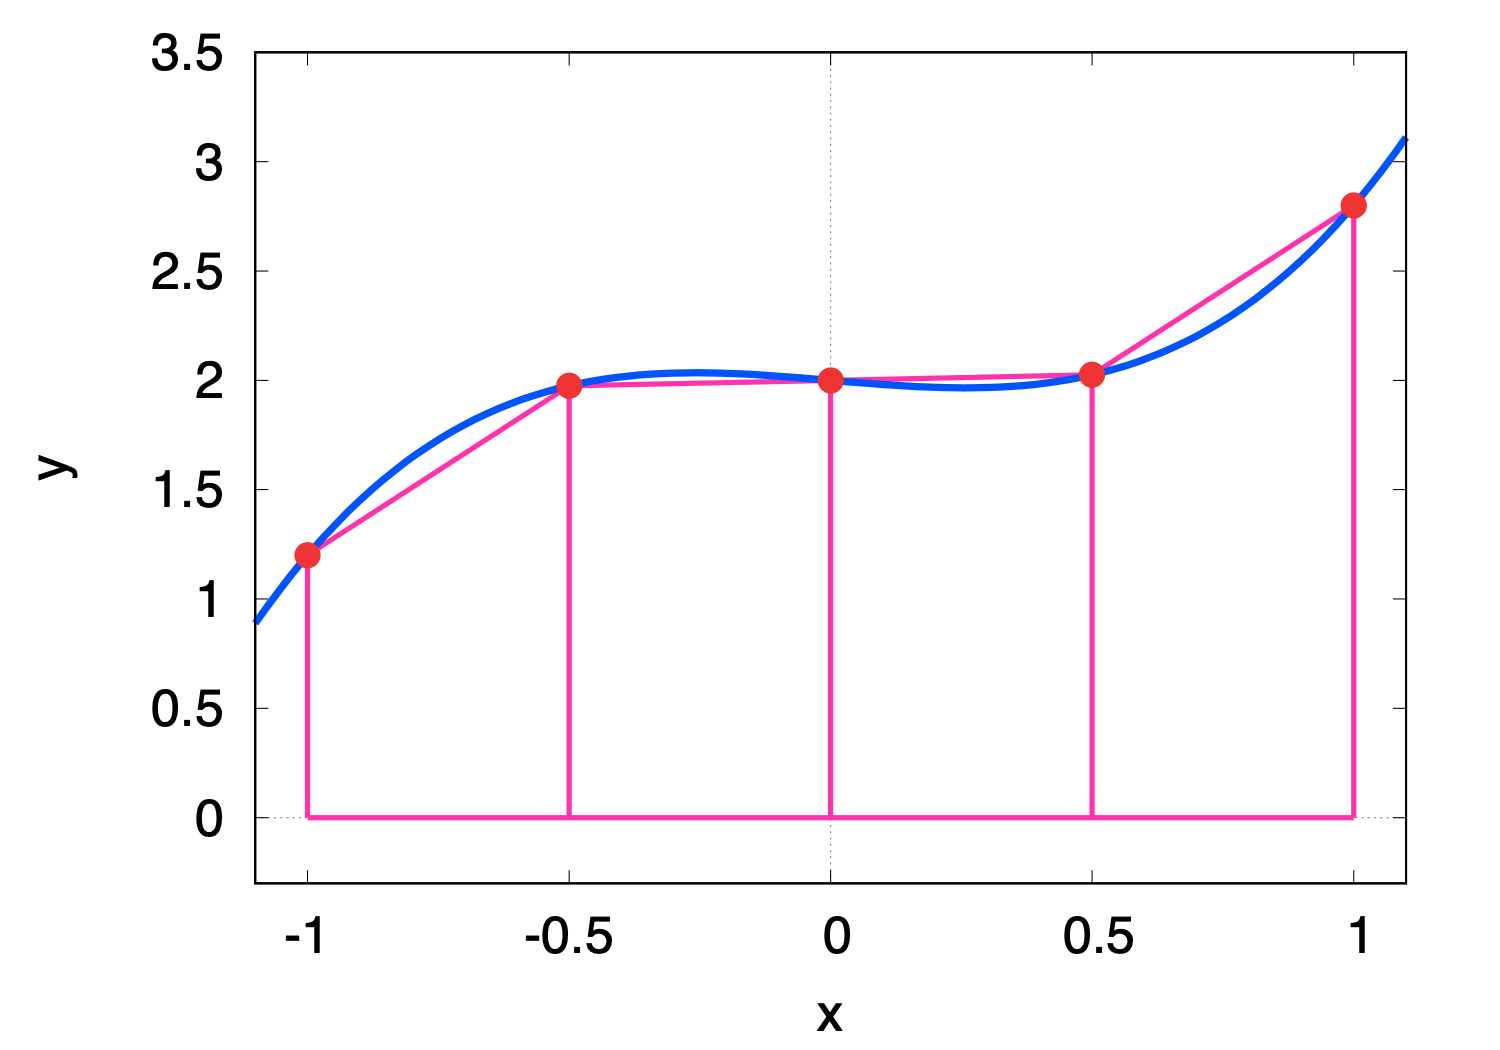
\includegraphics[width=1.0\textwidth]{fig11-1_trapezoid_rule_N4.png}
	\end{center}
	\vspace{-9mm}
	\caption{\myfontsetting{10pt}{10pt}{1次の区分的補間多項式でつないだ場合 ({\bf 複合的台形則})}}
\end{figure}
\end{column}
\end{columns}
\end{frame}
%%%%%%%%%%%%%%%%%%%%%%%%%%%%%%%%
\begin{frame}
\frametitle{\large [手法解説]}
\begin{block}{{\bf 数値積分法} {\small (Numerical Integration)}}
\myfontsetting{14pt}{16pt}{
関数 $f(x)$ の定積分 \myfontsetting{12pt}{12pt}{
$I = \displaystyle \int_a^b f(x) dx$
} を近似的に求める方法。
$N+1$ 個の{\bf 積分点} $x_i$ \myfontsetting{10pt}{10pt}{
$(0\le i \le N)$
} に対する関数の値 $f(x_i)$ に重み $\alpha_i$ をかけて足し上げた
\myfontsetting{12pt}{12pt}{
$\displaystyle I_N=\sum_{i=0}^N \alpha_i f(x_i)$
}
を数値的に求めて $I$ の近似値とする。
}
\end{block}

\vspace{-2mm}

\begin{itemize}
    %\setlength{\itemsep}{0.5cm}
    \item \myfontsetting{14pt}{16pt}{$\alpha_i$ の取り方によって $I_N$ の精度が異なる}
    %\begin{itemize}
    %    \item 複合台形則
    %    \item シンプソン則
    %\end{itemize}
    \item \myfontsetting{14pt}{16pt}{積分点を等間隔に取る方法は{\bf ニュートン・コーツ則} (Newton-Cotes rule) と呼ばれる}
\end{itemize}
\end{frame}
%%%%%%%%%%%%%%%%%%%%%%%%%%%%%%%%
\begin{frame}
\frametitle{数値積分法の種類}
\begin{itemize}
    \setlength{\itemsep}{0.5cm}
    \item {\bf 複合台形則} \myfontsetting{15pt}{15pt}{(Composite trapezoid rule)}
    \begin{itemize}
        \item \myfontsetting{15pt}{15pt}{隣り合う積分点を直線でつないだ関数の積分で近似
        }
        \item \myfontsetting{15pt}{15pt}{区間毎に見ると台形の面積を足し上げている
        }
        \item \myfontsetting{15pt}{15pt}{刻み幅 $h$ に対して $\mathcal{O}(h^2)$ の誤差}
    \end{itemize}
    \item {\bf シンプソン則} \myfontsetting{15pt}{15pt}{(Simpson's rule)}
    \begin{itemize}
        \item
        \myfontsetting{15pt}{15pt}{3点の積分点を放物線でつないだ関数の積分で近似}
        \item 
        \myfontsetting{15pt}{15pt}{刻み幅 $h$ に対して $\mathcal{O}(h^4)$ の誤差}
    \end{itemize}
\end{itemize}
\end{frame}
%%%%%%%%%%%%%%%%%%%%%%%%%%%%%%%%
\begin{frame}
\frametitle{[問題] X\hspace{-.1em}I-A}

%%%%% START_TAG A %%%%%
%\noindent{\bf [X\hspace{-.1em}I. 数値積分法]}%RETURN

%\noindent{\bf X\hspace{-.1em}I-A.}
\myfontsetting{15pt}{18pt}{
定積分 $\displaystyle \int_0^1 (e^x+1) dx$ を考える。\\
(1) 上記の定積分を計算しネイピア数 $e$ を用いて表せ。\\
(2) 上記の定積分を複合台形則を用いて数値積分する問題を考える。ニュートン・コーツ則で台形近似を行う区間の数を $N=2^n$ (積分点の数は $N+1=2^n+1$) とした時 の $n\ge 0$ を1ずつ増やして積分値を求めるプログラムを作成し、数値積分の値の相対誤差が $10^{-8}$ を下回る最も小さい $n$ を求めよ。
}\\
\myfontsetting{12pt}{12pt}{
作成したプログラムも提出すること。プログラミング言語は問わない。
}
%%%%% END_TAG A %%%%%
\end{frame}
%%%%%%%%%%%%%%%%%%%%%%%%%%%%%%%%
\begin{frame}
\frametitle{[略解] X\hspace{-.1em}I-A}
%\vspace{-0.5cm}
(1) $e$

\vspace{0.5cm}

(2) $n=12$

\end{frame}
%%%%%%%%%%%%%%%%%%%%%%%%%%%%%%%%
\begin{frame}
\frametitle{{\large [手法] 複合台形則} \myfontsetting{15pt}{18pt}{(Composite trapezoid rule)}}
    \begin{block}{{\bf\small 積分点を等間隔に取った複合台形則}}
        \myfontsetting{15pt}{18pt}{
        \begin{algorithmic}[1]
            \REQUIRE $f(x)$, $a$, $b$, $N$
            \ENSURE $I$
            \STATE $h \leftarrow \frac{b-a}{N}$
            \STATE $I \leftarrow \frac{1}{2}f(a)$
            \FOR{$j=1,2,\dots,N-1$}
            \STATE $I \leftarrow I + f(a+h\times j)$
            \ENDFOR
            \STATE $I \leftarrow I + \frac{1}{2}f(b)$
            \STATE $I \leftarrow I \times h$
        \end{algorithmic}
        }
    \end{block}
\end{frame}
%%%%%%%%%%%%%%%%%%%%%%%%%%%%%%%%
\begin{frame}
%%%%% PASTE_START_TAG B %%%%%
%\noindent{\bf X\hspace{-.1em}I-B.}
\frametitle{[問題] X\hspace{-.1em}I-B}

\myfontsetting{18pt}{18pt}{
X\hspace{-.1em}I-A で示した定積分をシンプソン則を用いて数値積分する問題を考える。ニュートン・コーツ則で2次多項式近似を行う区間の数を $M=2^{n-1}$ (積分点間の区画の数は $2M=2^n$、積分点の数は $2M+1=2^n+1$) とした時の $n\ge 1$ を1ずつ増やして積分値を求めるプログラムを作成し、数値積分の値の相対誤差が $10^{-8}$ を下回る最も小さい $n$ を求めよ。
}\\
\myfontsetting{12pt}{12pt}{
作成したプログラムも提出すること。プログラミング言語は問わない。
}
%%%%% PASTE_END_TAG B %%%%%
\end{frame}
%%%%%%%%%%%%%%%%%%%%%%%%%%%%%%%%
\begin{frame}
\frametitle{\myfontsetting{28pt}{28pt}{シンプソン則の図解}}
\begin{columns}[t]
\begin{column}{0.55\textwidth} 
\vspace{-5mm}
\begin{itemize}
    \setlength{\itemsep}{0.25cm}
    \item \myfontsetting{15pt}{17pt}{積分点3点を通る2次の補間多項式をつなげた曲線下の面積を積分の近似値として用いる}
    \begin{itemize}
        \item \myfontsetting{12pt}{12pt}{実際に補間多項式の係数を求める必要はない}
    \end{itemize}
\end{itemize}
\end{column}
\begin{column}{0.45\textwidth} 
\begin{figure}[h]
	\begin{center}
\vspace{-12mm}
    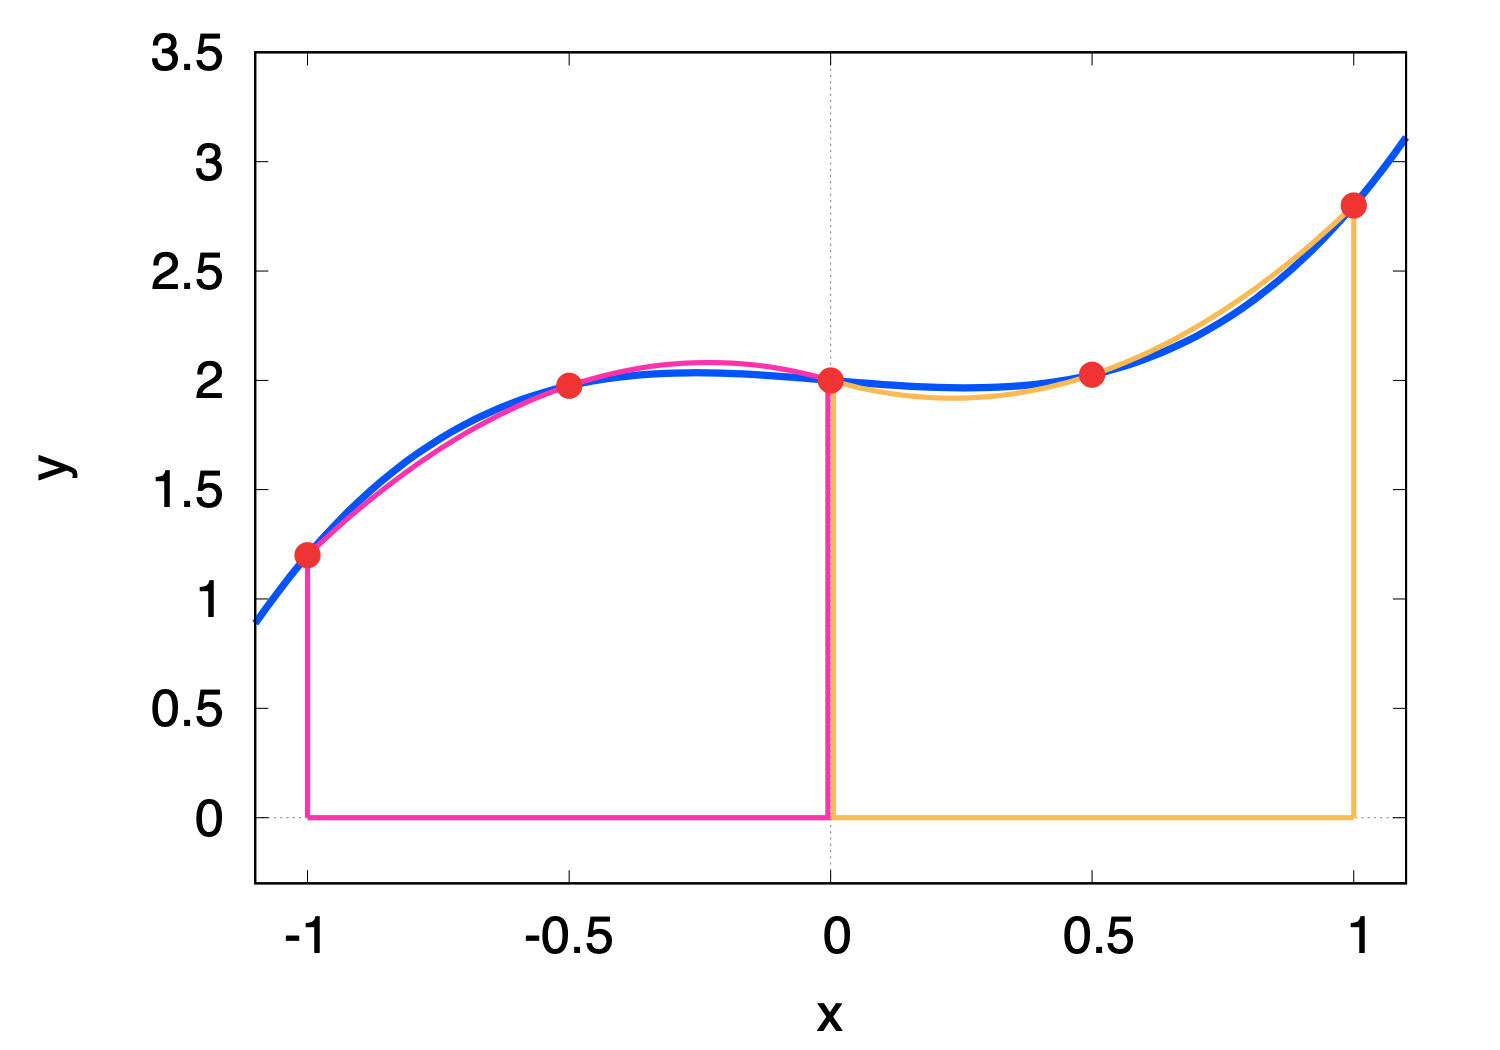
\includegraphics[width=1.0\textwidth]{fig11-2_simpson_rule_N4.png}
	\end{center}
	\vspace{-5mm}
	\caption{\myfontsetting{10pt}{10pt}{2次の区分的補間多項式でつないだ場合 ({\bf シンプソン則})}}
\end{figure}
\end{column}
\end{columns}
\end{frame}
%%%%%%%%%%%%%%%%%%%%%%%%%%%%%%%%
\begin{frame}
\frametitle{{\large [手法] シンプソン則} \myfontsetting{15pt}{18pt}{(Simpson's rule)}}
    \begin{block}{{\bf\small 積分点を等間隔に取ったシンプソン則}}
        \myfontsetting{12pt}{18pt}{
        \begin{algorithmic}[1]
            \REQUIRE $f(x)$, $a$, $b$, $M$ \myfontsetting{8pt}{8pt}{
            [$f(x_i)$ \myfontsetting{6pt}{6pt}{$(0\le i \le 2M)$} の重み付きの和を考える。$M=1$ の時 $\ell.$~\ref{op:second_for} のfor文はスキップ] }
            \ENSURE $I$
            \STATE $h \leftarrow \frac{b-a}{2M}$
            \STATE $I \leftarrow \frac{1}{3}f(a)$
            \FOR{$j=1,3,\dots,2M-1$}
            \STATE $I \leftarrow I + \frac{4}{3} f(a+h\times j)$
            \ENDFOR
            \FOR{$j=2,4,\dots,2M-2$ \label{op:second_for}}
            \STATE $I \leftarrow I + \frac{2}{3}f(a+h\times j)$
            \ENDFOR
            \STATE $I \leftarrow I + \frac{1}{3}f(b)$
            \STATE $I \leftarrow I \times h$
        \end{algorithmic}
        }
    \end{block}
\end{frame}
%%%%%%%%%%%%%%%%%%%%%%%%%%%%%%%%
\end{document}
